\documentclass{article}
\usepackage{graphicx}
\usepackage{makecell}
\usepackage[T1]{fontenc}
%\usepackage{tgpagella}      
\usepackage[dvipsnames]{xcolor}
\usepackage{booktabs}
\usepackage{comment}
\usepackage{longtable}
\usepackage{tgpagella} 
\usepackage{xfrac} 
\usepackage{float} 
\usepackage{colortbl}
\usepackage{hyperref}
\RequirePackage{fontawesome}
\usepackage{hyperref}
\hypersetup{
    colorlinks=true, 
    linktoc=all,     
    linkcolor=black!80,
    filecolor=blue,
    urlcolor=cyan!80
}
\usepackage{geometry}
\geometry{a4paper, total={5.5in, 9in}}
\renewcommand{\arraystretch}{1.4}
\newcommand{\must}{\cellcolor{Green}{M}}
\newcommand{\should}{\cellcolor{LimeGreen}{S}}
\newcommand{\could}{\cellcolor{RedOrange}{C}}
\newcommand{\wont}{\cellcolor{BrickRed}{W}}

\title{\huge Gestione del Progetto}
\author{Gabriele Chignoli}
\date{Maggio 2025}
\begin{document}
\maketitle
\tableofcontents
\newpage

\section{Ciclo di Vita del Software}
Dopo un'analisi dei principali modelli disponibili per la modellazione del ciclo di vita del software, si è giunti alla conclusione che sia gli approcci "pesanti" che quelli più agili hanno utili proprietà che vanno combinate per portare ad un processo più, secondo il team, completo e "umano".  \newline 

Dei processi pesanti, viene considerata la pianificazione iniziale fondamentale a garantire che il progetto si mantenga nel tempo all'interno di binari definiti e, preferibilmente, solidi. Tuttavia si considera che tale processo rischi di diventare troppo morboso e vincolante; in particolare l'impossibilità di tornare ad operare su fasi iniziali già completate, viene vista come una grande limitazione. 

Per questi motivi è stato deciso di adottare il \textbf{\textit{Modello a Cascata}} come modello base per la produzione del progetto; in aggiunta si intende concedere al team di  "risalire la cascata" ogni qualvolta sia necessario (credendo nel fatto che le risalite diminuiscano con l'avanzamento del progetto) e di quanti step si vuole, adottando così alcuni aspetti caratteristici di un approccio più iterativo, e quindi in parte anche più agile. Infine, si considerano le tre fasi finali di implementazione, testing e manutenzione (che include il refactoring) come un processo continuo in cui ogni parte è fondamentale per la seguente, e necessita di quella che l'ha preceduta. Si ritiene dunque che una visione e rappresentazione più ciclica di tali fasi sia più adatta. \newline 

Tenendo in mente queste accortezze, si è tentato di rappresentare anche graficamente il modello adottato:

\begin{figure}[H]
    \centering
    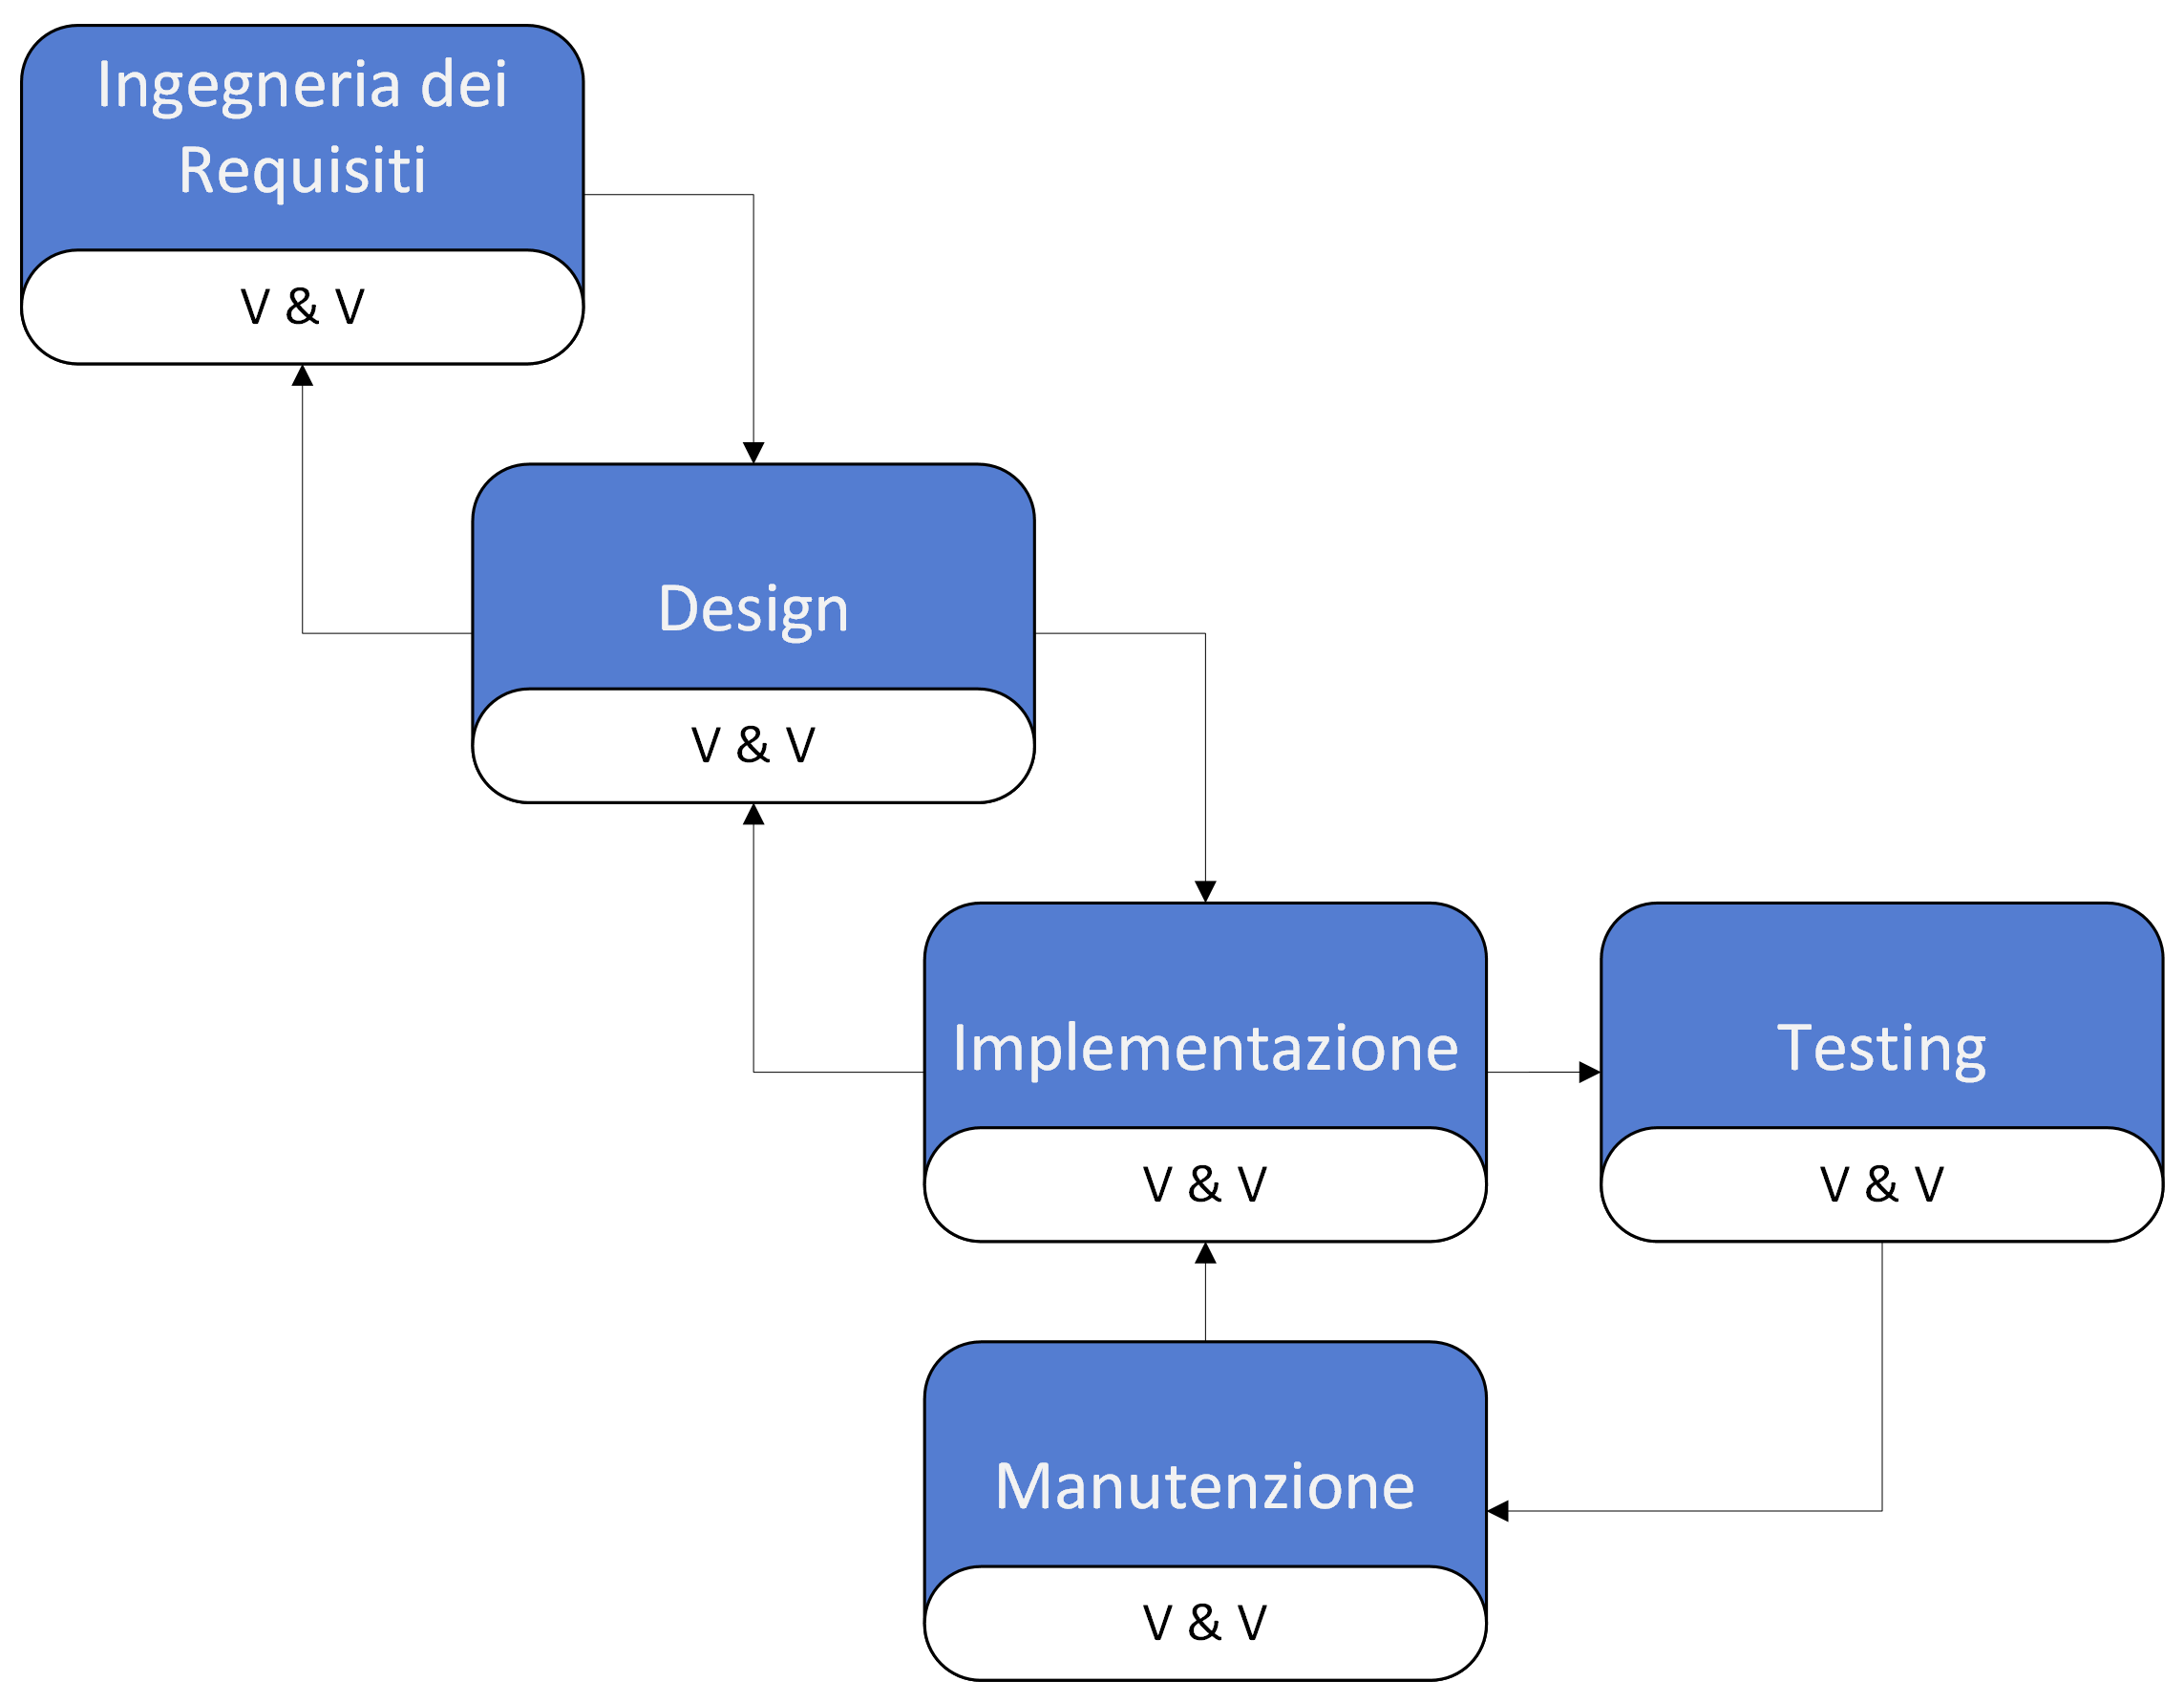
\includegraphics[width=.8\linewidth]{imgs/Modello a Cascata_0.png}
    \caption{Modello a Cascata Modificato}
    \label{fig:enter-label}
\end{figure}



\section{Configuration Management}
Il progetto utilizza per la gestione della configurazione la piattaforma \textbf{\textit{GitHub}}, della quale si intendono utilizzare le principali funzionalità disponibili. Inoltre si utilizzerà la \textbf{\textit{Kanban Board} }messa a disposizione nella sezione \textit{Progetti} di \textit{GitHub}, con la quale tenere traccia dei compiti e del loro stato. 

\section{People Management}
Pur essendo composto attualmente da un solo membro, verrà comunque simulata la presenza di un secondo sviluppatore (sempre controllato dallo sviluppatore principale). Si procede dunque a stabilire l'organizzazione del team secondo la quale si intende operare. \newline 

Date le dimensioni del progetto abbastanza contenute e il tipo di personale disponibile (studenti universitari), si ritiene che la struttura più adatta per lo svolgimento del compito sia un'\textbf{Organizzazione a Matrice}. In tal modo, tutti i membri possono operare su diverse (anche tutte) parti del progetto e quindi imparare, facendo, come costruire un software nella sua completezza, dalla documentazione e progettazione, al testing e all'implementazione, sfruttando questo ambiente "sandbox", invece che avere effettive responsabilità come nel mondo lavorativo. \newline 

\paragraph{Allocazione lavoro al 24/05/2025}
Le principali aree di lavoro e la loro allocazione al personale attuale sono elencate nella seguente tabella:
\begin{center}
    \begin{longtable}{ccc}
    \toprule
         %\rowcolor{NavyBlue!70}
         \textbf{Area di Lavoro} & \textbf{Personale}  & \\
         \midrule
         & Gabriele Chignoli & \dots \\
    \midrule
         Documentazione & $100\%$  & \dots \\
         Interfaccia Grafica & $100\%$ & \dots  \\
         Logica dell'applicazione & $100\%$ & \dots \\
         Testing & $100\%$  & \dots \\
         Data Base & $100\%$  & \dots \\
         Manutenzione & $100\%$ & \dots  \\
    \bottomrule
    \end{longtable}
\end{center}

\paragraph{Allocazione lavoro al 01/08/2025}
\begin{center}
    \begin{longtable}{ccc}
    \toprule
         %\rowcolor{NavyBlue!70}
         \textbf{Area di Lavoro} & \multicolumn{2}{c}{\textbf{Personale}} \\
         \midrule
         & Gabriele Chignoli & Developer \#2 \\
    \midrule
         Documentazione & $80\%$  & $20\%$ \\
         Interfaccia Grafica & $50\%$ & $50\%$  \\
         Logica dell'applicazione & $80\%$ &  $20\%$\\
         Testing & \dots  & $100\%$ \\
         Data Base & $100\%$  & \dots \\
         Manutenzione & $50\%$ & $50\%$  \\
    \bottomrule
    \end{longtable}
\end{center}

\paragraph{Commenti su allocazione effettiva - 04/09/2025}
Non è stato possibile tener traccia delle effettive percentuali di lavoro esercitate da ogni membro. Sarebbe stato utile introdurre un sistema di \textit{\#tag} da utilizzare per i commit (o per i branch) in modo da poter contare il numero di commit per membro per area di lavoro. Si può notare comunque dalle statistiche ottenute da \textit{Github} che vi è un forte squilibrio, principalmente causato dall'entrata tardiva del secondo membro nello sviluppo.     

\begin{figure}[h]
    \centering
    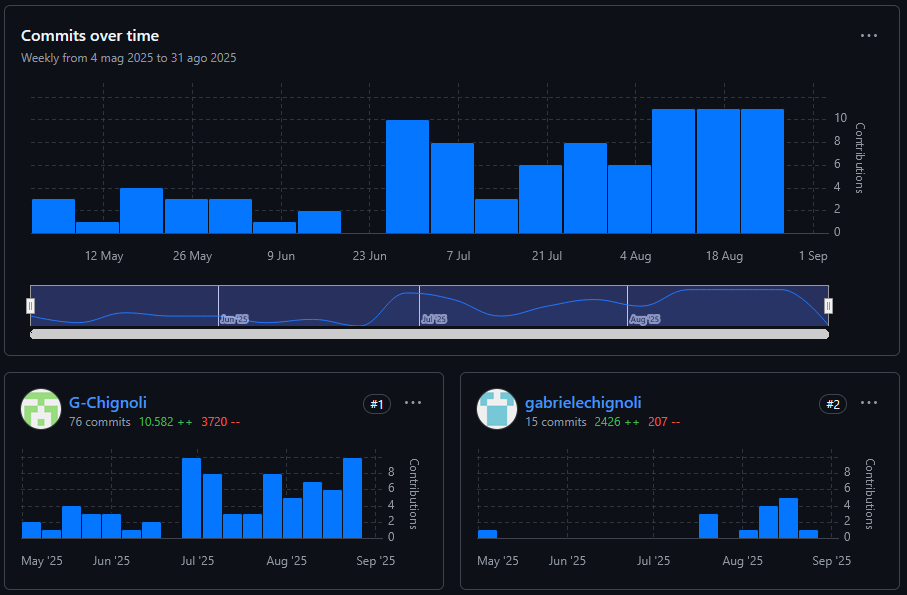
\includegraphics[width=\textwidth]{imgs/commit.png}
    \caption{Statistiche Contributors Github}
    \label{fig:placeholder}
\end{figure}

Si stima che i risultati effettivi siano più in linea con la seguente tabella:

\begin{center}
    \begin{longtable}{ccc}
    \toprule
         %\rowcolor{NavyBlue!70}
         \textbf{Area di Lavoro} & \multicolumn{2}{c}{\textbf{Personale}} \\
         \midrule
         & Gabriele Chignoli & Developer \#2 \\
    \midrule
         Documentazione & \color{green}$100\%$  & \color{red}\dots \\
         Interfaccia Grafica & \color{red}$20\%$ & \color{green} $80\%$  \\
         Logica dell'applicazione & $80\%$ &  $20\%$\\
         Testing & \color{green}$40\%$  & \color{red}$60\%$ \\
         Data Base & $100\%$  & \dots \\
         Manutenzione & $50\%$ & $50\%$  \\
    \bottomrule
    \end{longtable}
\end{center}


\end{document}
